\documentclass[11pt]{article}

%%%%%%%%%%%%%%Include Packages%%%%%%%%%%%%%%%%%%%%%%%%%%
\usepackage{xcolor}
\usepackage{mathtools}
\usepackage[a4paper, total={6in, 8in}, margin=1.25in]{geometry}
\usepackage{amsmath}
\usepackage{amssymb}
\usepackage{paralist}
\usepackage{rsfso}
\usepackage{amsthm}
\usepackage{wasysym}
\usepackage[inline]{enumitem}   
\usepackage{hyperref}
\usepackage{tocloft}
\usepackage{titlesec}
\usepackage{colortbl}
\usepackage{wrapfig}
\usepackage{pdfpages}
%%%%%%%%%%%%%%%%%%%%%%%%%%%%%%%%%%%%%%%%%%%%%%%%%%%%%%%%



\begin{document}
%\begin{wrapfigure}[8]{r}{0.3\textwidth}
%  \begin{center}
%  \vspace{-15pt}
%    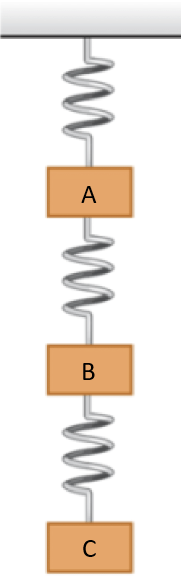
\includegraphics[scale=0.45]{springboxes}
%  \end{center}
%\end{wrapfigure}
\Large \noindent \textbf{Physics 1A Discussion (Week 6)}\\
\normalsize
Department of Physics and Astronomy, UCLA\\
\noindent\rule{8cm}{0.4pt}\\
Jinyan invented a launch machine as shown. Two identical springs are attached to a plate and he is trying to launch a pumpkin using this launcher. Jinyan spends $500\,$N to pull the plate a distance $\Delta x = 2$\,m from the equilibrium position of the launcher. Then he releases the plate to launch the $1\,$kg pumpkin. Neglect friction in this problem.\\
\begin{center}
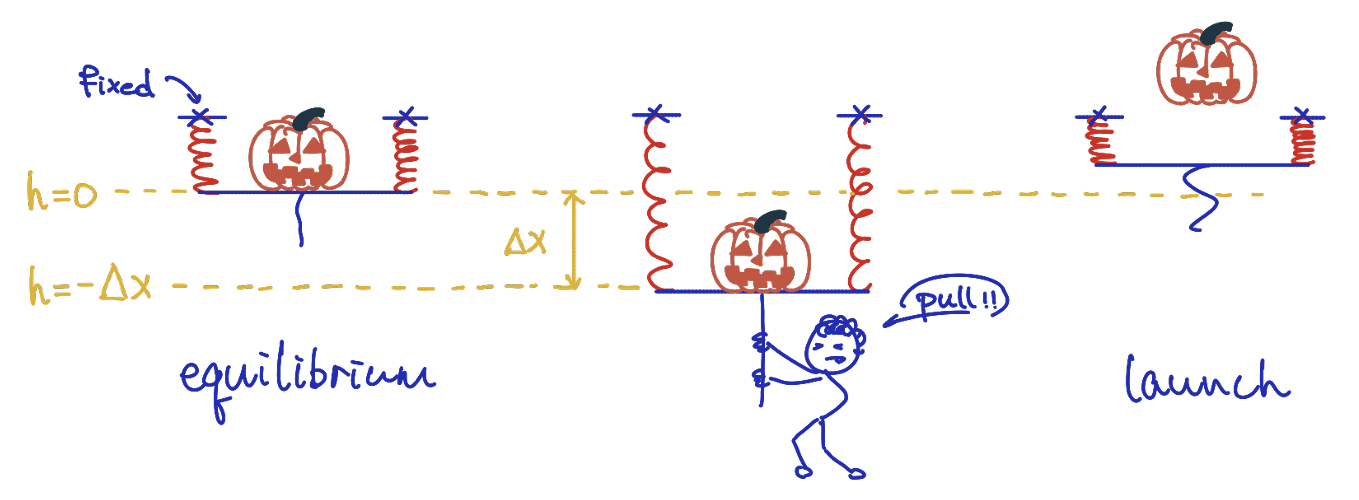
\includegraphics[scale=0.35]{launch}
\end{center}


\noindent (a) Find the speed of the pumpkin when the launcher is back to its equilibrium position.\\

\noindent (b) Find the maximum height that the pumpkin can reach.\\

\noindent (c) If the pumpkin is launched at an angle as shown (assuming that it leaves the launcher with the same speed $|\vec{v}_i|$ as computed in part (a)), find the angle $\theta$ relative to the ground such that Jinyan can launch the pumpkin to reach a maximum height of $30$\,m. \\

\begin{center}
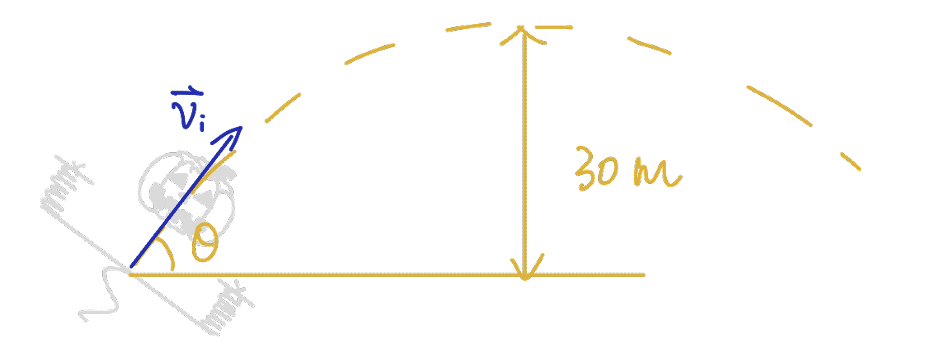
\includegraphics[scale=0.35]{angle}
\end{center}



\vfill
\noindent\textbf{Hint}: \color{gray} 
For part (a), first compute the spring constant of the springs. Then apply energy conservation. Part (b) is a straightforward application of energy conservation. Part (c) is a little tricky, Pythagoras said $v^2 = v_x^2 + v_y^2$, and we can use that in our application of energy conservation. 
\color{black}



%\newpage
%\textbf{Solutions}: First we find the spring constant of the springs. At equilibrium, some spring forces already balance the weight of the pumpkin, and since spring force is linear in displacement of the spring, we do not need to consider the effect due to the weight of the pumpkin when we use $\Delta x$ to find the spring constant: Apart from equilibrium, the spring forces balance the $500\,\text{N}$ applied force by Jinyan acting on the plate. Since the springs are identical, we can say each spring provides a spring force of $250\,$N, from which we can find the spring constant, 
%\begin{align*}
%250\,\text{N} = |F_{\text{spring}}| = k\, \Delta x = k \cdot (2\,\text{m})\,.
%\end{align*} 
%Thus we have $k = 125 \,$N/m. Now we write the statement of energy conservation, 
%\begin{align*}
%E_{\text{initial}} + W_{\text{external}} = E_{\text{final}}\,.
%\end{align*}
%Each of the energies $E$ can be broken down into two parts: the kinetic energy $K$ and the potential energy $U$. $W_{\text{external}}$ is the work done by any external force (this could be friction, applied force, or some other factors), but we don't have any of those once Jinyan releases the plate, so $W_{\text{external}} = 0$. The potential energies that are involved in this problem include the gravitational potential energy $U_g = mgh$ and the spring potential energy $U_k = (k/2)(\Delta x)^2$. \footnote{In other words, the gravitational potential energy accounts for the work done by the gravitational force, and the spring potential energy accounts for the work done by the spring force.} \\
%
%For part (a), we pick the initial point to be the time instant where plate is released, and the final point to be the time instant where the launcher is back to equilibrium. 
%\begin{align*}
%E_{\text{initial}}&= E_{\text{final}}\,,\\
%\frac{1}{2}mv_i^2 + \frac{1}{2}k(\Delta x_i)^2+ \frac{1}{2}k(\Delta x_i)^2+mgh_i &=
%\frac{1}{2}mv_f^2 + \frac{1}{2}k(\Delta x_f)^2+ \frac{1}{2}k(\Delta x_f)^2+mgh_f\,. 
%\end{align*}
%At initial time, $\Delta x_i = \Delta x$, $v_i = 0$ (pumpkin starts from rest), and $h_i = -\Delta x$ (the plate is pulled back by $\Delta x$). At final time, $\Delta x_f = 0$ (launcher back to equilibrium position), $v_f$ is the final speed we want to find, and $h_f = 0$ (at equilibrium). Thus we have
%\begin{align*}
%k(\Delta x)^2 -mg\,\Delta x = \frac{1}{2}m v_f^2 \,,
%\end{align*}
%from which we find
%\begin{align*}
%v_f = \sqrt{\frac{2k}{m}(\Delta x)^2 - 2g\,\Delta x}=31.0\,\text{m/s} \,.
%\end{align*}
%Now part (b), we pick the initial point to be the time instant where the launcher is back to equilibrium (which is the final point in part (a)), and we pick the final point to be the time instant where the pumpkin reaches its maximum height. In this process, the pumpkin has left the launcher, and thus the spring potential energy is no longer relevant. We only need to consider the gravitational potential energy and the kinetic energy, 
%\begin{align*}
%E_{\text{initial}}&= E_{\text{final}}\,,\\
%\frac{1}{2}mv_i^2 +mgh_i &=
%\frac{1}{2}mv_f^2 +mgh_f\,.
%\end{align*}
%At the initial point, $v_i = 31.0\,\text{m/s}$ as computed in part (a), $h_i = 0$ by how we set up the axes. At the final point $v_f =0$ because the pumpkin has reached its maximum height and wants to ``turn around" from going up to going down, $h_f$ is the quantity that we want to find. Thus we have
%\begin{align*}
%\frac{1}{2}m v_i^2 = mgh_f\,,
%\end{align*}
%from which we find 
%\begin{align*}
%h_f = \frac{v_i^2}{2g} = 49.0\,\text{m}\,.
%\end{align*}
%Lastly, for part (c), we pick the final point to be the time instant where the pumpkin reaches its maximal height again, but in this case, we no longer have $v_f = 0$ because the projectile motion of the pumpkin has a nonzero constant $v_x$ throughout its whole path. Instead, we can write $v_x^2 + v_y^2 = v^2$ for both the initial and the final velocity. At the final position, the $y$-component of the final velocity vanishes, and the $x$-component of the final velocity is exactly the same as the $x$-component of the initial velocity (because there is no acceleration in the $x$-direction), thus 
%\begin{align*}
%E_{\text{initial}}&= E_{\text{final}}\,,\\
%\frac{1}{2}mv_i^2 +mgh_i &=
%\frac{1}{2}mv_f^2 +mgh_f\,,\\
%\frac{1}{2}m(v_{i,x}^2+v_{i,y}^2) +mgh_i &=
%\frac{1}{2}m(v_{f,x}^2+v_{f,y}^2) +mgh_f\,,\\
%\frac{1}{2}m(v_{i,x}^2+v_{i,y}^2) +mgh_i &=
%\frac{1}{2}mv_{i,x}^2 +mgh_f\,,
%\end{align*}
%therefore, 
%\begin{align*}
%\frac{1}{2}mv_{i,y}^2 &=
%mgh_f\,.
%\end{align*}
%We have the initial velocity from part (a), so we can calculate its $y$-component via $v_y = v_i \sin(\theta)$. Now plug in everything, 
%\begin{align*}
%\frac{1}{2}mv_i^2 \sin^2(\theta) = mg h_f\,,
%\end{align*}
%from which we get
%\begin{align*}
%\theta = \arcsin\left(\sqrt{
%\frac{2gh_f}{v_i^2}
%}\right)=0.900\, \text{rad} = 51.55^\circ\,.
%\end{align*}



\end{document}


